%!TEX root = ../MasterThesis.tex

\chapter{Concept and Design of the System} % (fold)
\label{cha:design_system}

This chapter will \ldots

\section{Overview}
\label{sec:system_overview}

Based on the explanations in Section~\ref{cha:context_analysis}, and especially the scope definition for this Master thesis in Section~\ref{sec:scope_thesis}, the system for investigating E-commerce fraud incidents have to answer the central question:\@

\begin{quotation}
    \textit{Is this really a fraudulent E-commerce transaction?}
\end{quotation}

The main stakeholders, that need to be involved in the investigation process are:\@

\begin{itemize}
    \item the online merchants
    \item the \gls{PSP}
    \item the issuer
\end{itemize}

Ideally they would make part of their internal information available for external partners to access and query for, so that the party, who has to authorize or validate the credit card payment can analyse all available information, as depicted in the Figure~\ref{fig:images_system_overview}.

\begin{figure}[H]
	\centering
		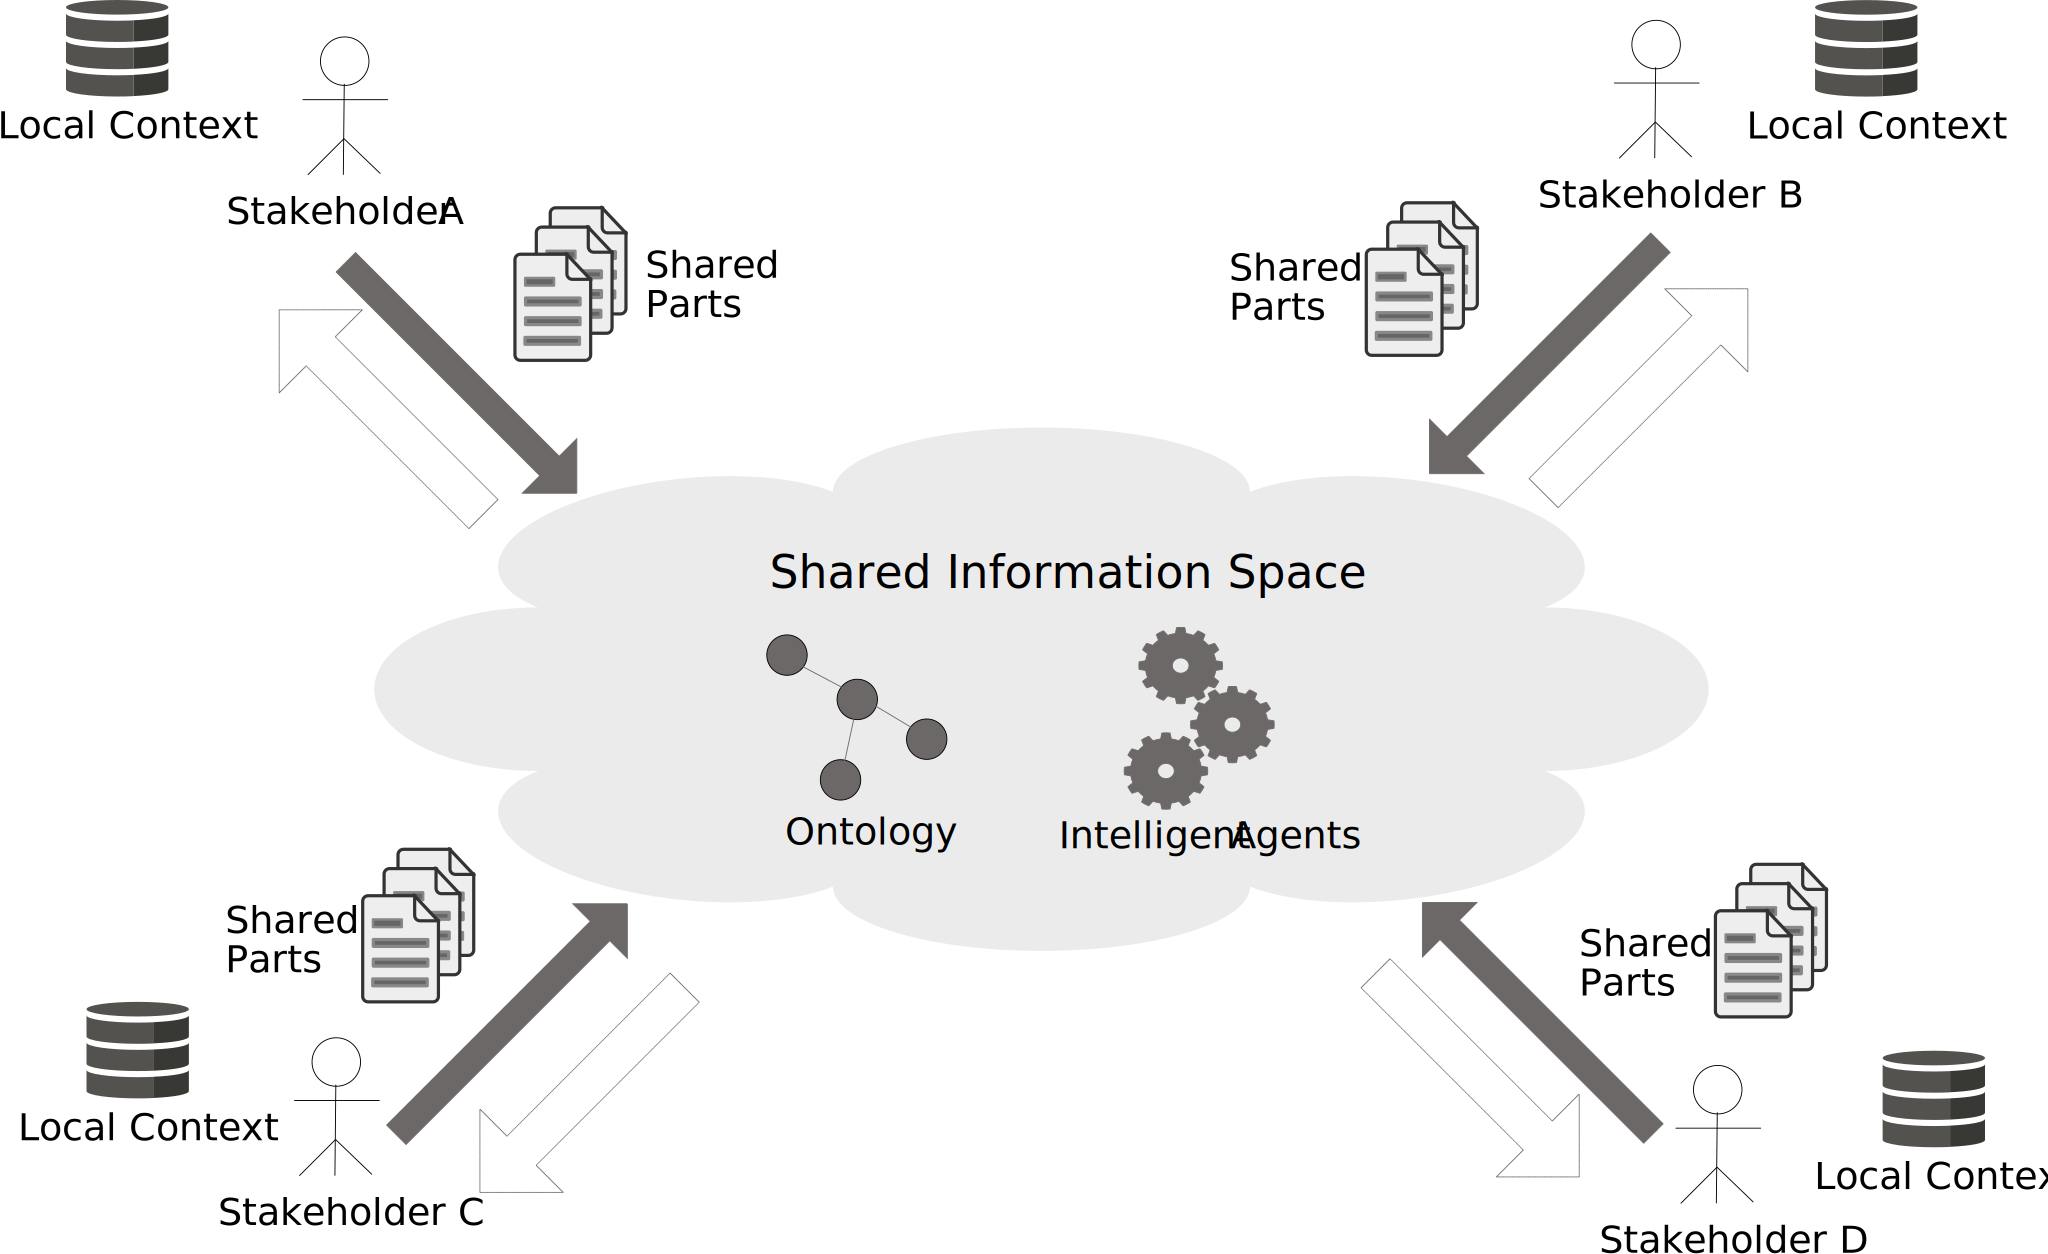
\includegraphics[width=0.8\columnwidth]{images/system_overview.pdf}
	\caption{System Overview}
\label{fig:images_system_overview}
\end{figure}

\ldots

% section system_overview (end)

\section{Initial Approaches}
\label{sec:system_approaches}

When trying to solve issues of information integration between organisations there are already existing solutions, that have to be examined whether they might fit the E-commerce fraud investigation scenario or not.

\subsection{Web of Services}
\label{subsec:web_services}

With the development of the E-commerce scenario there was also a need to integrate business functionality from various service providers operating on the Internet. Good examples for this are the integration of the \gls{PSP} into the payment as well as the \gls{LSP} for the shipping process. These approaches resulted in the ``Service Oriented Architecture'' paradigm, that enables application services provided by different vendors to talk to each other via a public facing programming interface (aka \gls{API}). The only requirement for such interoperability to work properly is, that each public interface follows some standardised or commonly agreed upon guidelines to be vendor-, platform- as well as language-agnostic. One possible implementation of these concepts are the so-called Web Services, that use the WS* protocols and standards from the \gls{W3C} with the extensible markup language (aka \gls{XML}) and the \gls{HTTP} protocol at their core \citep{josuttis2007soa}. \\

Like the \gls{HTML} format, that is used to represent Web pages on the Internet, \gls{XML} is originally based on \gls{SGML}, but instead of formalising markup tags for structuring and styling textual content it is a meta-language allowing everyone to define his or her own markup languages. In this matter it doesn’t dictate what tags are available to structure the information; instead it includes some basic guidelines for creating wellformed and valid documents that uses domain-specific tags, which can be freely defined and structured by the creator of the XML document. Therefore it is better suited in situations where a computer has to parse and evaluate the content of a message (assuming the computer program knows the structure of the message) \\

In an additional step the author of the API could also specify an XML schema for each message, which describes the structure of the message with all the possible elements, their ordering, nesting level and data types in detail. By doing so the XML parser program can later verify the content of a retrieved message against the XML schema and check if it is a valid document (related to the schema definition). XML schematas are also expressed in XML format and have been standardised by the W3C. Being able to create custom markup languages via XML has a huge benefit for machine-to-machine communication and is the basis for integrating Web Services (via the WS* protocols), but it still has limitations when it comes to figure out the semantics of those XML messages. This is mostly due to the fact that each XML document represents a new markup language and needs a specific XML parser to be understood by the machine; also to distinguish commonly used tag names in an XML document the creator has to place them into specific namespaces (aka XML namespaces). But those XML namespaces further complicate the automatic processing of XML documents and increases the necessity to have custom instances of XML parsers for each XML document \citep{taylor2008p2p}. \\



% subsection web_services (end)

\subsection{Web of Data}
\label{subsec:web_data}

``The Web is full of intelligent applications, with new innovations coming every day.'' But each of those intelligent Web applications is driven by the data available to them. Data that is likely coming from different places in the global information space — accessible usually via a custom API on the server hosting those resources (see Section~\ref{subsec:web_services}). The more consistent the data available to the smart Web application is the better the service and its result will be. But to support an integration of the data from various Web services the semantics of the information delivered by each service has to be available — and there has to be a generalised, formalised way to express the semantic of that data. The focus on a standard that allows Web services to express the semantics of the data they provide also allows for global scalability, openness and decentralisation, which are the key principles of the World-Wide Web. The Semantic Web tries to give a solution for this problem by providing the Resource Description Framework (aka \gls{RDF}) and related technologies (e.g. RDF schema, SPARQL, OWL, \ldots) for describing, linking and querying the data that a Web service delivers. But it doesn’t reinvent the wheel; instead the Semantic Web builds upon existing, proven technologies like XML, XML namespaces, XML schemata and the \gls{URI} to uniquely address resources on the Web \citep{allemang2011semantic}. \\

% subsection web_data (end)

\subsection{Conclusion and Findings}
\label{subsec:conclusion_findings}

% section conclusion_findings

% section system_approaches (end)

\section{Concept and Design}
\label{sec:concept_design}

% section concept_design (end)

% chapter design system (end)
